\documentclass[11pt]{article}
\usepackage[T1]{fontenc}
\usepackage{lmodern}
\usepackage[utf8]{inputenc}
\usepackage[margin=1in]{geometry}
\usepackage{amsmath,amssymb,amsthm,mathtools}
\usepackage{graphicx,booktabs,array,microtype}
\usepackage{xcolor}
\usepackage[colorlinks=true,linkcolor=blue!55!black,citecolor=teal!60!black,urlcolor=blue!55!black]{hyperref}
\setlength{\emergencystretch}{2em}
\newtheorem{theorem}{Theorem}[section]
\newtheorem{proposition}[theorem]{Proposition}
\newtheorem{lemma}[theorem]{Lemma}
\theoremstyle{remark}
\newtheorem{remark}[theorem]{Remark}
\newcommand{\R}{\mathbb R}
\newcommand{\C}{\mathbb C}
\newcommand{\N}{\mathbb N}
\newcommand{\PF}{\mathrm{PF}}
\newcommand{\code}[1]{\nolinkurl{#1}}
\DeclareMathOperator{\Rea}{Re}
\DeclareMathOperator{\Ima}{Im}
\title{\bfseries How sensitive are finite RH criteria?\\Certified Davenport--Heilbronn controls}
\author{Biswajit Mondal}
\date{Working draft, October 13, 2026}
\begin{document}
\maketitle
\begin{abstract}
Finite positivity tests related to the Riemann Hypothesis require calibration
against functions with known off-line zeros. We study the classical
Davenport--Heilbronn function, additional character combinations, and two
Epstein zeta functions. An argument-principle computation certifies the complete
Davenport--Heilbronn zero atlas through height 340: 235 critical-line zeros and
seven reflected off-line pairs in the upper half-plane. A leading-term
Dirichlet-series bound proves that the zero at height \(85.69934849\) has the
largest folded angular deviation among all zeros. Schoenberg's sufficient
sector theorem consequently gives \(\PF_{435}\) for the ordinary folded
Taylor coefficients. Nevertheless, all 18,291 contiguous minors at ranks
430--520 and shifts 0--200 are positive at 32,768-bit precision. The isolated
quadratic factor first has a negative shift-one minor at rank 436.
An elementary masking lemma explains why such a factor need not force failure
in a fixed-shift ladder; a dominant-pole argument proves eventual positivity
of the full Davenport--Heilbronn shift-one ladder.
We also give certified negative geometric-form trials
for seven controls, including a conductor-17 test of a prediction recorded
before its new window search, and finite-zero-sum attribution diagnostics.
The window data are negative-support upper bounds, not certified minimum
supports. Neither the fitted calibration nor the finite Toeplitz grid yields
a universal zero-free region or a proof of the Riemann Hypothesis.
\end{abstract}
\noindent\textbf{Keywords:} Davenport--Heilbronn function; Weil quadratic form;
Toeplitz minors; total positivity; interval arithmetic; negative controls;
zero detection.

\noindent\textbf{MSC 2020:} 11M26, 11M41, 15B05.

\section{Introduction}
An all-orders positivity criterion can characterize the Riemann Hypothesis
without making a finite instance a sensitive detector of an off-line zero.
The distinction matters when choosing a finite computational target.
Davenport--Heilbronn functions supply controls with a functional equation and
zeros off the symmetry line. Their classical theory and numerical zero
computations are established background
\cite{dh1936,balanzario2007,bombieriGhosh2011}.
All seven off-line centers in Table~\ref{tab:dhzeros} were already reported:
the first four by Spira and the final three by Balanzario--S\'anchez-Ortiz,
as recorded in \cite{balanzario2007}. Our contribution is the complete
interval count and global angular comparison, rather than discovery of
these zero locations.

Our main result is a reproducible calibration for one specified family of
Toeplitz minors. We certify the steepest folded Davenport--Heilbronn zero and
the resulting \(\PF_{435}\) sufficient guarantee, then test the requested
grid beyond the isolated quadratic's first negative minor. Every tested
full-function minor is positive. This is a failure of sharpness for the
specified solid grid. It does not locate the globally first negative minor,
and does not prove \(\PF_{520}\).

The window experiments address a different finite criterion. We construct
rational trial functions with negative Weil-type quadratic form directly
from the geometric side. The existing \texttt{teal-sea/zeta-lab} report
\cite{teal2026} already found the classical Davenport--Heilbronn negative
window near \(C=31\); that observation is prior work. We refine the
finite-family search, add other controls, and distinguish the resulting
upper bounds from a theorem about the minimum negative support.
Bombieri's fixed-support spectral analysis \cite{bombieri2000} is direct
prior art for this finite-to-infinite distinction.

The contributions of this draft are:
\begin{itemize}
\item a complete interval-certified Davenport--Heilbronn atlas through height
340 and a global steepest-angle reduction;
\item a fully resolved 18,291-cell solid-minor grid, with a second determinant
identity checking selected high-rank cells;
\item a common-degree seven-control window calibration, a recorded
conductor-17 prediction test, and enclosed finite-atlas quartet contributions;
\item an elementary fixed-shift masking lemma and a direct eventual-positivity
argument for the classical Davenport--Heilbronn shift-one ladder.
\end{itemize}
These are calibration results. The analytic reductions use classical
functional equations, factorization and sector theorems; the numerical
enclosures use Arb. They have not undergone independent external review.

\section{Normalizations and the finite tests}\label{sec:normalization}
\subsection{Character combinations and Epstein controls}
Let \(\chi\) be a primitive odd nonreal character of conductor \(q\), and put
\begin{equation}\label{eq:character}
 \epsilon_\chi=\frac{\tau(\chi)}{i\sqrt q},\qquad
 \kappa_\chi=\frac{\Ima\epsilon_\chi}{1+\Rea\epsilon_\chi},\qquad
 H_\chi(s)=\frac{(1-i\kappa_\chi)L(s,\chi)
                    +(1+i\kappa_\chi)L(s,\bar\chi)}2.
\end{equation}
We exclude the singular normalization \(1+\Rea\epsilon_\chi=0\).
The Dirichlet coefficients are real, periodic, and have first coefficient
one. The completion
\begin{equation}\label{eq:completion}
 \Lambda_\chi(s)=(q/\pi)^{s/2}\Gamma((s+1)/2)H_\chi(s)
\end{equation}
is entire and satisfies \(\Lambda_\chi(s)=\Lambda_\chi(1-s)\).
The classical control has \(q=5\), \(\chi(2)=i\), and period
\((0,1,\kappa,-\kappa,-1)\), where
\begin{equation}\label{eq:dhkappa}
 \kappa=\frac{\sqrt{10-2\sqrt5}-2}{\sqrt5-1}.
\end{equation}
We also use \(H_d(s)=E(s,x^2+dy^2)/2\), \(d=5,6\), normalized by
counting representations. The class-number-two decompositions are
\begin{align}
 H_5(s)&=\tfrac12\{\zeta(s)L(s,\chi_{-20})
                         +L(s,\chi_{-4})L(s,\chi_5)\},\label{eq:epstein5}\\
 H_6(s)&=\tfrac12\{\zeta(s)L(s,\chi_{-24})
                         +L(s,\chi_{-3})L(s,\chi_8)\}.\label{eq:epstein6}
\end{align}
Here \(\chi_D\) is the primitive quadratic character of fundamental
discriminant \(D\). The completion has gamma factor
\((\sqrt d/\pi)^s\Gamma(s)\) and poles at 0 and 1.
The entire symmetric target is therefore
\(s(s-1)(\sqrt d/\pi)^s\Gamma(s)H_d(s)\).
The contour computation uses \(F_d(s)=(s-1)H_d(s)\), removing the pole at 1;
the prefactor relating it to the entire target introduces no additional
zero inside the contours used here. Genus decompositions and their
normalizations are checked against independent representation counts.
The background for these controls is discussed in \cite{bombieriGhosh2011}.

\subsection{Ordinary coefficients and solid minors}
For the classical completion define the folded entire function
\begin{equation}\label{eq:fold}
 \frac{\Lambda_5(1/2+z)}{\Lambda_5(1/2)}
       =F(z^2),\qquad F(w)=\sum_{n\ge0}\mu_n w^n,\qquad \mu_0=1.
\end{equation}
All Toeplitz tests use the ordinary coefficients \(\mu_n\).
The classical Jensen coefficients \(n!\mu_n\) are different data and are
not substituted into these matrices. With \(\mu_n=0\) for \(n<0\), write
\begin{equation}\label{eq:solid}
 D_{r,s}=\det(\mu_{s+i-j})_{0\le i,j<r},
 \qquad D_{0,s}=D_{r,0}=1.
\end{equation}
\(\PF_m\) means nonnegativity of all Toeplitz minors of order at most \(m\),
including arbitrary row and column sets. Our solid grid is only a subset.

\subsection{Quadratic forms and support}
We use physical support \([-S/2,S/2]\), with
\begin{equation}\label{eq:support}
 S=\log C.
\end{equation}
For a real trial function let
\(\mathcal F_f(z)=\int_{-S/2}^{S/2}f(x)e^{zx}\,dx\).
The spectral form associated with a real symmetric completion is
\begin{equation}\label{eq:spectral}
 Q_H(f)=\sum_\rho \mathcal F_f(\rho-\tfrac12)
                  \overline{\mathcal F_f(\tfrac12-\bar\rho)}.
\end{equation}
Its geometric form uses the coefficients in
\(-H'/H=\sum_{n\ge2}c_n n^{-s}\).
For a character combination these coefficients need not have prime-power
support or one sign. All active integers \(n<C\) are included.
The odd gamma factor and conductor term in \eqref{eq:completion} are used,
and there is no pole block. The Epstein forms have their own gamma and pole
terms. The gamma duplication identity is used before reusing entry formulas.

The finite trial family consists of normalized cosines through order \(N\)
in the even sector and normalized sines through order \(N\) in the odd
sector, together with the constant even mode. Each sector is orthonormal in
\(L^2[-S/2,S/2]\). Stored coordinates use the shifted exponentials
\(S^{-1/2}e^{2\pi i n(x+S/2)/S}\), so the real centered sine and cosine modes
include the phase \((-1)^n\). This phase is retained in zero-side evaluation.
An interval LDL factorization proposes a rational vector at
its first negative leading pivot. The full geometric Rayleigh quotient of
that exact vector is then enclosed independently of the pivot sign.
A negative quotient proves a negative full-form trial.
Positivity of the finite matrix proves only positivity on that finite space.
The spaces obtained by changing \(S\) are not nested, so the searches below
do not provide monotone brackets for the first negative full support.

\section{The complete classical Davenport--Heilbronn atlas}
\begin{lemma}[Positive theta kernel]\label{lem:theta}
The classical completion is positive on the real axis. Every ordinary
folded coefficient \(\mu_n\) is strictly positive.
\end{lemma}
\begin{proof}
Set \(\theta(t)=\sum_{n\ge1}na_n e^{-\pi n^2t/5}\).
Poisson summation for the odd character combination gives
\(\theta(t)=t^{-3/2}\theta(1/t)\).
For \(t\ge1\), put \(v=\pi t/5>1/2\). Since \(a_2=\kappa>0\) and
\(|a_n|\le1\),
\begin{equation}\label{eq:thetabound}
 \theta(t)\ge e^{-v}-\sum_{n\ge3}n e^{-vn^2}
 \ge e^{-v}-\frac{e^{-4v}}{2v}>0.
\end{equation}
The middle inequality uses the decreasing function \(x e^{-vx^2}\) on
\([2,\infty)\). Consequently \(\Psi(u)=e^{3u/2}\theta(e^{2u})\) is even and
positive. Mellin inversion gives
\begin{equation}\label{eq:thetamellin}
 \Lambda_5(1/2+z)=4\sqrt{\pi/5}\int_0^\infty\Psi(u)\cosh(zu)\,du.
\end{equation}
The kernel decays faster than any exponential. This proves real-axis
positivity and positivity of every even Taylor moment.
\end{proof}

\begin{theorem}[Computer-assisted atlas and steepest angle]\label{thm:atlas}
The completed classical Davenport--Heilbronn function has precisely 249
zeros, counted with multiplicity, in the upper half-plane through height
340. They consist of 235 critical-line zeros and seven reflected off-line
pairs. All are simple. Every completed zero satisfies
\(|\Rea\rho-\tfrac12|<1\). The zero near
\(0.8085171825+85.69934849i\) has the largest folded angular deviation among
all completed zeros.
\end{theorem}
\begin{proof}[Proof with explicit numerical inputs]
The first coefficient of \(H_5\) is one, and Arb gives
\begin{equation}\label{eq:tailstrip}
 \sum_{n\ge2}|a_n|n^{-3/2}=0.7375906494\ldots<1.
\end{equation}
The sum decreases with the real part. Thus \(H_5\) has no zero at
\(\Rea s\ge3/2\); the completed functional equation gives the reflected
exclusion at \(\Rea s\le-1/2\).
There are no gamma poles inside this strip.

On the rectangle \([-1/2,3/2]+i[0,340]\), the real bottom has zero argument
increment by Lemma~\ref{lem:theta}; its gamma factor is positive there.
The other three sides are covered by 5,208 Taylor image rectangles excluding
zero. A convex zero-excluding image gives a continuous argument increment
of magnitude less than \(\pi\), so principal endpoint increments may be
summed. Their total encloses \(2\pi\cdot249\).
There are 235 disjoint critical-line sign brackets and seven disjoint simple
right-hand Rouché disks. Functional-equation reflection supplies seven
left-hand disks. Their multiplicity count exhausts 249, proving completeness
and simplicity. The atlas is replayed at higher precision with additional
subdivision where needed.

For \(\rho=1/2+b+i\gamma\), the zero of \(F\) at
\(w=(\rho-1/2)^2\) has angular deviation
\begin{equation}\label{eq:angle}
 \phi_\rho=2\arctan\frac{|b|}{|\gamma|}
\end{equation}
from the negative axis. The height-85.6993 disk has
\(\phi=0.0071999578790\ldots\), greater than the deviations of all other
off-line disks and greater than \(2\arctan(1/340)\).
The strip exclusion therefore controls every higher zero as well.
Every comparison uses enclosing balls, rather than the rounded values in
Table~\ref{tab:dhzeros}.
\end{proof}

\begin{table}[ht]
\centering
\caption{Right-hand classical Davenport--Heilbronn zeros below height 340.
The reflected zeros and 235 critical-line zeros exhaust the contour count.
Rounded coordinates are not certificate inputs.}\label{tab:dhzeros}
\begin{tabular}{rr}
\toprule \(\Rea\rho\) & \(\Ima\rho\)\\ \midrule
0.8085171825 & 85.69934849\\
0.6508300806 & 114.1633427\\
0.5743560505 & 166.4793059\\
0.7242576946 & 176.7024612\\
0.8695305796 & 240.4046724\\
0.8195495921 & 320.8764897\\
0.7682231236 & 331.0502594\\
\bottomrule
\end{tabular}
\end{table}

\section{The sector guarantee and the high-rank grid}
\begin{theorem}[Sufficient sector guarantee]\label{thm:pf}
The ordinary coefficient sequence in \eqref{eq:fold} belongs to
\(\PF_{435}\).
\end{theorem}
\begin{proof}
The folded function has order \(1/2\), hence a genus-zero product with
constant one. By Theorem~\ref{thm:atlas} every zero lies in the wedge about the
negative axis of half-angle \(\phi\), where interval calculation gives
\begin{equation}\label{eq:ratio}
 436<\frac{\pi}{\phi}=436.3348656172\ldots<437.
\end{equation}
Schoenberg's sufficient sector theorem, stated as Theorem B in
\cite{katkova2005}, gives \(\PF_{435}\) for every finite conjugation-invariant
product prefix: its wedge half-angle is less than \(\pi/436\).
The prefixes converge locally uniformly. Each fixed Toeplitz minor is a
polynomial in finitely many coefficients, so nonnegativity passes to the
entire function.
\end{proof}
For the isolated quadratic \(A(w)=1+2\cos\phi\,w+w^2\), expansion of the
tridiagonal determinant gives
\begin{equation}\label{eq:chebyshev}
 D_{r,1}(A)=U_r(\cos\phi)=\frac{\sin((r+1)\phi)}{\sin\phi}.
\end{equation}
Equation~\eqref{eq:ratio} makes rank 436 its first negative shift-one minor.
The angular rank scale is \(\pi|\gamma|/(2|b|)\), retaining the offset \(b\).

\begin{proposition}[Certified solid grid]\label{prop:grid}
For the full folded Davenport--Heilbronn function,
\(D_{r,s}>0\) for every \(430\le r\le520\) and \(0\le s\le200\).
\end{proposition}
\begin{proof}[Computational verification]
We generate 721 ordinary coefficients through index 720 at 32,768 bits.
The positive rescaling \(\mu_n\mapsto100^n\mu_n\) preserves determinant signs.
Desnanot--Jacobi condensation evaluates
\begin{equation}\label{eq:condensation}
 D_{r,s}=\frac{D_{r-1,s}^2-D_{r-1,s-1}D_{r-1,s+1}}{D_{r-2,s}}.
\end{equation}
Every divisor is required to exclude zero; unresolved entries invalidate
their descendants. All 18,291 requested cells resolve positive.
This count includes the 91 trivial shift-zero cells.
The full sign digest is replayed.
For \(h_n=[w^n]1/F(-w)\), Jacobi's complementary-minor identity also gives
\begin{equation}\label{eq:complement}
 D_{r,s}=\det(h_{r+i-j})_{0\le i,j<s}.
\end{equation}
It independently checks 24 high-rank cells at ranks
430, 435, 436, 437, 480 and 520, and shifts 1, 2, 5 and 20.
These checks share the interval coefficient input and FLINT backend, while
bypassing the condensation divisions.
\end{proof}
Figure~\ref{fig:grid} displays the distinction between the isolated factor
and the full-function grid. The sufficient sector bound is not sharp for
this tested family. Arbitrary row and column sets and larger shifts remain
untested, so Proposition~\ref{prop:grid} supplies no global first-failure
rank or \(\PF_{520}\) claim.

\begin{figure}[ht]
\centering
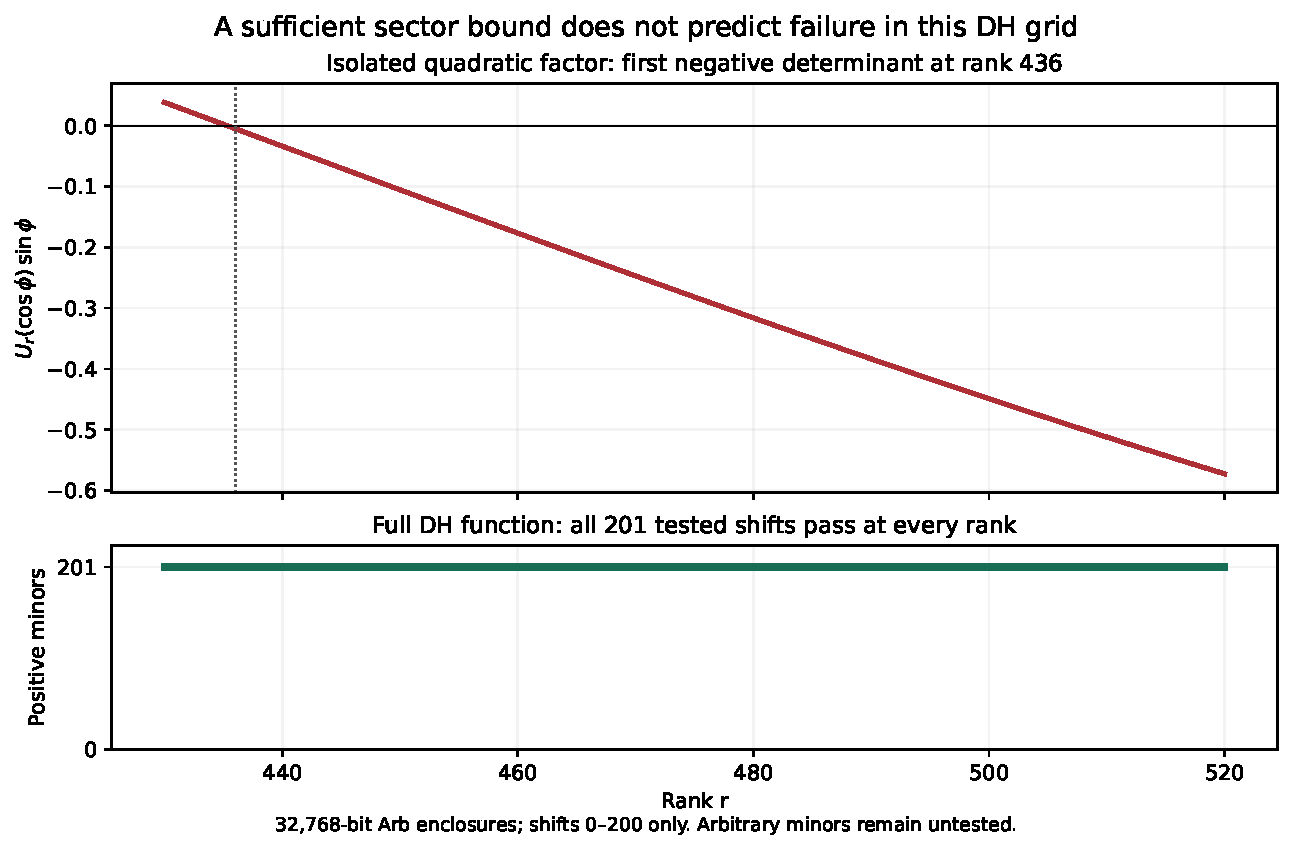
\includegraphics[width=\linewidth]{../research/prime_spectral/verification_2026_10_12_sector/dh_sector_grid.pdf}
\caption{The isolated quadratic determinant, scaled by \(\sin\phi\), changes
sign at rank 436. Every one of the 201 tested full-function shifts remains
positive at each rank through 520. The lower panel counts signs; it does not
compare determinant magnitudes or assert positivity of arbitrary minors.}
\label{fig:grid}
\end{figure}

\section{Why multiplication can conceal a negative factor}
Toeplitz multiplication and Cauchy--Binet expand a product minor into a sum
of products of factor minors. One negative term need not determine the sum.
The following elementary example makes that obstruction quantitative.
It is included as an explanation, without a novelty claim.

\begin{lemma}[A fixed-shift ladder can miss a conjugate pair forever]\label{lem:mask}
Let \(0<c<1\) and
\begin{equation}\label{eq:mask}
 G(w)=(1+4w)(1+2cw+w^2).
\end{equation}
Then \(G\) has two nonreal zeros, yet
\begin{equation}\label{eq:maskbound}
 D_{r,1}(G)\ge \frac29\,4^r>0\qquad(r\ge0).
\end{equation}
\end{lemma}
\begin{proof}
The two nonreal zeros belong to the quadratic, while \(1+4w\) adds a
negative real zero. The reciprocal generating identity gives
\begin{equation}\label{eq:maskseries}
 D_{r,1}(G)=[w^r]\frac1{G(-w)}
       =\sum_{j=0}^r4^{r-j}U_j(c).
\end{equation}
Writing \(c=\cos\phi\) with \(0<\phi<\pi/2\), the finite exponential sum for
\(U_j(\cos\phi)\) gives \(|U_j(c)|\le j+1\).
Since \(U_0=1\),
\begin{equation}\label{eq:maskestimate}
 4^{-r}D_{r,1}(G)
 \ge1-\sum_{j=1}^{\infty}\frac{j+1}{4^j}
 =2-(1-\tfrac14)^{-2}=\frac29.
\end{equation}
\end{proof}
This lemma concerns one fixed-shift ladder. Other minors of \(G\) may fail.
It does not prove the full Davenport--Heilbronn grid by factorization, since
the remaining Davenport--Heilbronn factors include further off-line pairs.
It explains why the first negative minor of an isolated quadratic is not an
upper bound for the corresponding full-function ladder.

\begin{proposition}[Eventual positivity of the DH shift-one ladder]\label{prop:dhmask}
Let \(\gamma_1\) be the lowest positive Davenport--Heilbronn zero ordinate
and put \(a=\gamma_1^2\). There is a constant \(A>0\) such that
\begin{equation}\label{eq:dhmask}
 D_{r,1}(F)=A a^{-r}+O(64^{-r})\qquad(r\longrightarrow\infty).
\end{equation}
In particular, the full-function shift-one minors are strictly positive
at every sufficiently large rank, despite the off-line zeros.
\end{proposition}
\begin{proof}
The complete atlas places the first two positive critical-line ordinates
in \((81/16,41/8)\) and \((143/16,9)\), respectively.
There is no off-line zero below height 85. Thus the first folded zero
\(-a\) is simple and unique in \(|w|\le64\), since
\((41/8)^2<64<(143/16)^2\).
Write \(B(w)=F(-w)\). We have \(B(0)=1\), and \(B\) is real and
nonzero on \([0,a)\). Its simple first crossing therefore has
\(B'(a)<0\). Set \(A=-1/(aB'(a))>0\).
The function
\[
 \frac1{B(w)}-\frac{A}{1-w/a}
\]
is analytic on a neighborhood of the closed disk \(|w|\le64\).
Cauchy's coefficient estimate and
\(D_{r,1}(F)=[w^r]1/B(w)\) prove \eqref{eq:dhmask}.
\end{proof}
This is ordinary dominant-pole analysis, included without a novelty claim.
It does not give an explicit last exceptional rank, prove positivity at
every rank, or control other shifts. It shows directly how a nearer real
zero can dominate this particular DH ladder.

\section{Seven-control window calibration}\label{sec:calibration}
We compare the finite-family negative endpoints at common degree \(N=192\)
and 2,048-bit arithmetic. Table~\ref{tab:calibration} reports the lowest
off-line zero from each complete finite atlas, the positive finite endpoint,
and the certified negative endpoint. Complete atlases reach height 160 for
the additional character combinations and 120 for the Epstein controls.
A conductor-11 exploratory combination has no off-line zero below 160 and
is excluded from the fitted seven-point sample.

The leading zero densities motivate a normalized resolution coordinate,
rather than an exchange theorem:
\begin{equation}\label{eq:resolution}
 T_*(C)=
 \begin{cases}
  2\pi C/q,&\text{odd character completion of conductor }q,\\
  \pi\sqrt{C/d},&\text{Epstein form }x^2+dy^2,
 \end{cases}
 \qquad r=\frac{T_*(C)}{\gamma}.
\end{equation}
These expressions equate the leading ordinate density with the exponential
type budget \(S/(2\pi)\). That calculation does not prove that an off-line
zero is detected at \(T_*(C)\).
\begin{table}[ht]
\centering
\small
\caption{Common-degree calibration, $N=192$. $C_+$ means positive finite evidence; $C_-$ is a certified negative full-form trial. The values are rounded; exact rational endpoints are retained in the supplement. $r=T_*(C_-)/\gamma$.}\label{tab:calibration}
\begin{tabular}{lrrrrr}
\toprule Control & $\gamma$ & $b$ & $C_+$ & $C_-$ & $r$\\\midrule
DH5 & 85.699348 & 0.308517 & 30.628746 & 30.630219 & 0.44914 \\
DH13(2) & 31.434205 & 0.083622 & 33.750244 & 33.751953 & 0.51896 \\
Epstein5 & 15.668250 & 0.432970 & 19.825439 & 19.827148 & 0.39928 \\
DH17(3) & 105.155287 & 0.163306 & 133.738281 & 133.751953 & 0.47011 \\
DH7(3) & 31.580361 & 0.535699 & 13.008621 & 13.010651 & 0.36980 \\
DH13(6) & 25.608746 & 0.362174 & 21.099091 & 21.101334 & 0.39825 \\
Epstein6 & 15.117579 & 0.303749 & 31.778137 & 31.781708 & 0.47828 \\
\bottomrule
\end{tabular}
\end{table}


Before the new conductor-17 window search, the prediction \(C=140\), with
the interval \([126,154]\), was recorded from the earlier three-control
calibration. Its atlas proves that
\(0.6633061848+105.15528688i\) is the lowest off-line zero.
The negative endpoint \(C=133.751953125\) is 4.46\% below the forecast
and falls inside the predicted interval.
Degree 80 remains positive at every tested point through
200, whereas degrees 128 and 192 give negative trials at 140.
Thus a detector-resolution check is necessary even for the empirical test.
At degree 256, the tested section is positive at \(C=133.5\) and a rational
witness is negative at \(C=133.73828125\). This modest change from degree
192 supports finite-family resolution stability at this control.
None of these positive sections certifies a positive full window.

Figure~\ref{fig:calibration} shows the seven finite-family upper-bound
coordinates and descriptive fits. The fitted samples are not independent
measurements of minimum support. The two Epstein observations offer only
limited information on a degree effect, and the conductor-7 control has a
zero to the right of 1. These distinctions limit extrapolation to zeta.
The simple fit \(r=a+kb\) has root-mean-square residual 0.0183.
Adding a degree term reduces it to 0.0149, but the largest absolute
leave-one-out error in the implied \(C\) rises from 16.3\% to 19.6\%.
Seven support upper bounds therefore do not establish a universal
10\%-accurate exchange law.
\begin{figure}[ht]
\centering
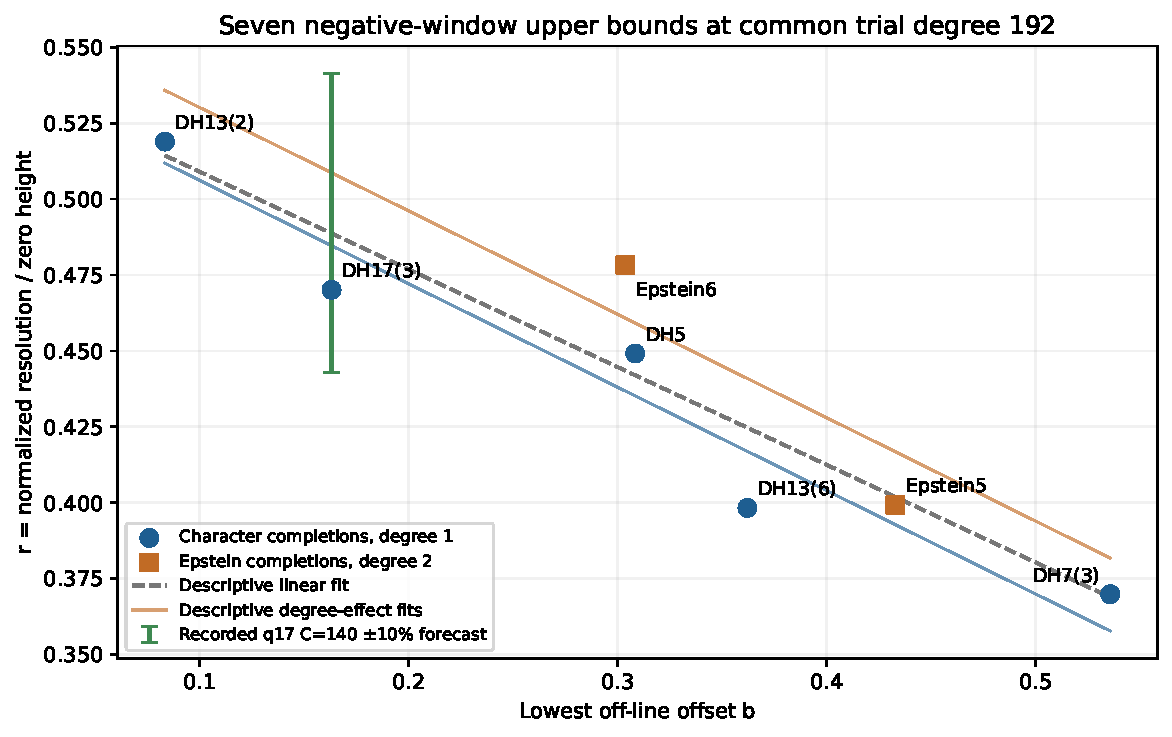
\includegraphics[width=.9\linewidth]{figures/dh_controls_calibration.pdf}
\caption{Normalized negative-window upper bounds \(r=T_*(C_-)/\gamma\)
against the lowest off-line offset \(b\), using common trial degree 192.
The fits are descriptive. They do not provide confidence intervals for
unknown minimum supports or a zero-free region for zeta. The conductor-17
prediction was supplied before the new window trials.}
\label{fig:calibration}
\end{figure}

\section{Finite-zero-sum attribution}
For a normalized real even witness, an off-line quartet represented by
\(z=b+i\gamma\) contributes
\begin{equation}\label{eq:quarteteven}
 4\Rea\{\mathcal F_f(z)^2\}.
\end{equation}
For a real odd witness the contribution has the opposite sign.
A critical-line pair contributes \(2|\mathcal F_f(i\gamma)|^2\).
We refine the atlas disks to radius \(10^{-120}\), verify containment in their
parent disks or sign brackets, and evaluate these finite contributions with
interval arithmetic.

Table~\ref{tab:attribution} identifies the largest enclosed
negative quartet contribution for each negative endpoint witness.
The supplementary records retain the positive line sum separately from
the finite total. This answers which
quartet carries the negative term within the atlas. It does not prove that
the omitted infinite tail is negligible at the scale of the geometric
quotient. The exact geometric certificate proves negativity; the finite
zero sum supplies mechanism evidence. A non-smooth Fourier witness does not
automatically give the tail decay needed to promote that evidence to an
independent full spectral certificate.
\begin{table}[ht]
\centering\small
\caption{Attribution for each common-degree negative endpoint witness. The dominant negative quartet is the lowest off-line pair in all seven finite atlases. $P_H$ is the sum over the complete atlas below height $H$; $Q$ is the certified geometric quotient. Their difference is material, so the finite sum is mechanism evidence rather than a negligible-tail spectral certificate.}\label{tab:attribution}
\begin{tabular}{lcrrr}
\toprule Control & Parity & Dominant $\gamma$ & $Q$ & $P_H$\\\midrule
DH5 & even & 85.699348 & $-9.772\times10^{-33}$ & $-2.519\times10^{-30}$\\
DH13(2) & even & 31.434205 & $-6.173\times10^{-17}$ & $-4.418\times10^{-13}$\\
Epstein5 & even & 15.668250 & $-1.031\times10^{-8}$ & $-1.296\times10^{-4}$\\
DH17(3) & even & 105.155287 & $-1.483\times10^{-43}$ & $-5.005\times10^{-40}$\\
DH7(3) & odd & 31.580361 & $-9.555\times10^{-10}$ & $-4.135\times10^{-6}$\\
DH13(6) & even & 25.608746 & $-3.045\times10^{-10}$ & $-8.222\times10^{-7}$\\
Epstein6 & even & 15.117579 & $-3.789\times10^{-9}$ & $-2.180\times10^{-5}$\\
\bottomrule
\end{tabular}
\end{table}


\section{Reproduction and limits of inference}
The code uses Python 3.12, python-flint 0.8.0, and Arb/FLINT interval
arithmetic. Discovery Newton steps and floating-point pilot scans select
candidates only. The accepted root disks, contour images, determinant signs,
Rayleigh quotients, and frequency panels are checked with outward
enclosures. The supplement records source hashes, input hashes, exact
rational trial coefficients, pivot intervals, and replay commands.
Regenerable full matrix arrays are omitted from compact records; the initial
generator is preserved by hash. Public archival release and external
analytic review are pending.

The classical atlas uses \code{dh_zero_atlas.py} and
\code{replay_dh_atlas.py}. The existing solid grid and complementary checks
use \code{dh_high_rank_scan.py} and \code{replay_dh_high_rank.py}; no further
Toeplitz grid is generated for this paper. New control atlases use
\code{character_zero_atlas.py} and \code{epstein_zero_atlas.py}.
The geometric calibration and finite attribution use
\code{control_window_calibration.py} and \code{control_zero_attribution.py}.

The finite Schur inertia identity after completion of the square and the
actual quadratic Toeplitz determinant formula are checked in Lean 4.
Their six-theorem audit uses only \texttt{propext},
\texttt{Classical.choice}, and \texttt{Quot.sound}.
The analytic explicit formulas, entire-function factorization, Schoenberg
sector theorem, and interval computations remain separate written and
computer-assisted dependencies.

The data support testing a calibrated detector. They do not establish
\emph{positivity at \(C\) excludes every off-line zero below approximately
\(12C\)}. Such an implication additionally requires a uniform theorem over
offsets, multiplicities, local zero configurations, and the infinite tail.
The present offsets are bounded away from zero; their fitted curve does
not determine the small-offset limit. Likewise, the solid-grid result does
not characterize all minors of a given rank. These controls provide no
independent confirmation of a new zeta window-positivity record and no route
to RH by themselves.

\section{Discussion}
Two finite criteria show different sensitivities. The Toeplitz grid remains
positive after the isolated factor becomes negative, and
Lemma~\ref{lem:mask} demonstrates an exact fixed-shift masking mechanism.
Proposition~\ref{prop:dhmask} proves eventual positivity for the classical
Davenport--Heilbronn shift-one ladder itself.
The window family produces negative rational witnesses at reproducible
cutoffs, with a conductor-17 negative endpoint inside its forecast range.
The shared feature is that resolution and the zero configuration must be
accounted for before interpreting a finite sign.

The near-term mathematical target is a quantitative detector with a proved
tail and cancellation bound. The near-term computational target is a
certificate whose full comparison cost is measured, including the
infinite complement. Calibration of either target requires controls such
as those used here. Neither replaces the missing all-support arithmetic
estimate.

\appendix
\section{Entry formulas and removable-point contour images}

Here are explicit formulas for regenerating the new finite matrices.
Put \(\omega_m=2\pi m/S\), \(b_k=2k+2\alpha\), where
\(\alpha=1/4\) or \(3/4\). The no-pole gamma entry is
\begin{align}
 G_\alpha(m,m)
 ={}&-\log\pi+\Rea\psi(\alpha-i\omega_m/2)
       +\frac{\Rea\psi'(\alpha-i\omega_m/2)}{2S}\notag\\
 &-\frac2S\sum_{k\ge0}e^{-b_kS}
                \frac{b_k^2-\omega_m^2}{(b_k^2+\omega_m^2)^2},\label{eq:archdiag}\\
 G_\alpha(m,n)
 ={}&-\frac{\Ima\psi(\alpha-i\omega_m/2)
                    -\Ima\psi(\alpha-i\omega_n/2)}{2\pi(m-n)}
 \notag\\
 &-\frac1{\pi(m-n)}\sum_{k\ge0}e^{-b_kS}
       \left(\frac{\omega_m}{b_k^2+\omega_m^2}
                    -\frac{\omega_n}{b_k^2+\omega_n^2}\right)
       \quad(m\ne n).\label{eq:archoff}
\end{align}
They follow by expanding the gamma kernel and integrating the shifted
Fourier correlations. Truncation before \(k=K\) has a uniform absolute error
\begin{equation}\label{eq:archtail}
 \varepsilon_{\alpha,K}
 \le \frac{2e^{-(2K+2\alpha)S}}
 {S(2K+2\alpha)^2(1-e^{-2S})}.
\end{equation}
For the character controls use \(G_{3/4}+\log(q)I\) and subtract the finite
log-derivative correlation sum. For the Epstein controls use
\(G_{1/4}+G_{3/4}+\log(4d)I\), the one pole block, and that control's
log-derivative correlation sum. Selected entries are checked against
adaptive integration of the original regularized geometric kernel.
The parity matrices also obey the exact divided-difference formulas
implemented in the generator.

For completeness, the genus identities
\eqref{eq:epstein5}--\eqref{eq:epstein6} can be obtained from the two
reduced ideal classes. Their forms are \((1,0,5),(2,2,3)\) at discriminant
\(-20\), and \((1,0,6),(2,0,3)\) at discriminant \(-24\).
Decompose the principal partial zeta function into the trivial class
character and the nontrivial genus character. The latter Euler products
factor as \(L(\chi_{-4})L(\chi_5)\) and
\(L(\chi_{-3})L(\chi_8)\), respectively. The unit group has order two,
giving the representation normalization \(E/2\).

The additional contours enclose all four sides, including the real bottom;
they do not assume the classical DH positive-theta lemma for another
control. FLINT's direct series evaluations on nonzero-radius cells
containing removable points can be indeterminate. We use analytic Taylor
images there. For a character combination with zero period sum,
partial summation gives
\(|H(s)|\le |s|\sum_{n<q}|a_n|/\Rea s\) for \(\Rea s>0\).
Thus \(M=3\sum_{n<q}|a_n|\) bounds \(|H|\) on \(|s-1|\le1/2\).
The Taylor remainder through order \(K\) on \(|s-1|\le r<1/2\) is at most
\begin{equation}\label{eq:cauchy}
 M\,\frac{(2r)^{K+1}}{1-2r}.
\end{equation}
For \(F_d=(s-1)H_d\), fractional-part partial summation gives
\(|(s-1)\zeta(s)|\le3\) on the same disk. If \(M_j\) are the three
character-period absolute sums in the genus decomposition, a valid bound is
\((9M_0+(9/2)M_1M_2)/2\).
Near zero the regular functional-equation identity is
\begin{equation}\label{eq:epsteinregular}
 F_d(s)=\frac{\Gamma(2-s)}{\Gamma(1+s)}
          (\sqrt d/\pi)^{1-2s}F_d(1-s).
\end{equation}
Cauchy bounds on a slightly larger Taylor disk also enclose the required
derivative coefficients. These images, ordinary Taylor images elsewhere,
and the Rouché inequalities are the numerical inputs to the finite zero
counts.

\begin{thebibliography}{99}
\bibitem{dh1936}
H. Davenport and H. Heilbronn,
On the zeros of certain Dirichlet series,
\emph{J. London Math. Soc.} \textbf{11} (1936), 307--312.
\href{https://doi.org/10.1112/jlms/s1-11.4.307}{doi:10.1112/jlms/s1-11.4.307}.
\bibitem{balanzario2007}
E. P. Balanzario and J. S\'anchez-Ortiz,
Zeros of the Davenport--Heilbronn counterexample,
\emph{Math. Comp.} \textbf{76} (2007), 2045--2049.
\href{https://doi.org/10.1090/S0025-5718-07-01999-0}{doi:10.1090/S0025-5718-07-01999-0}.
\bibitem{bombieriGhosh2011}
E. Bombieri and A. Ghosh,
Around the Davenport--Heilbronn function,
\emph{Russian Math. Surveys} \textbf{66} (2011), 221--270.
\href{https://doi.org/10.1070/RM2011v066n02ABEH004740}{doi:10.1070/RM2011v066n02ABEH004740}.
\bibitem{bombieri2000}
E. Bombieri,
Remarks on Weil's quadratic functional in the theory of prime numbers, I,
\emph{Rend. Lincei Mat. Appl.} \textbf{11} (2000), 183--233.
\url{https://www.bdim.eu/item?id=RLIN_2000_9_11_3_183_0}.
\bibitem{katkova2005}
O. M. Katkova,
Multiple positivity and the Riemann zeta-function,
arXiv:math/0505174 (2005), especially Theorem B.
\url{https://arxiv.org/abs/math/0505174}.
\bibitem{teal2026}
\texttt{teal-sea/zeta-lab},
Truncated Weil form: first positivity failure on Davenport--Heilbronn is at
\((c,N)=(31,60)\), tracking the off-line pair,
research report, GitHub issue 57, August 17, 2026.
\url{https://github.com/teal-sea/zeta-lab/issues/57}.
Accessed October 13, 2026.
\end{thebibliography}
\end{document}
